\PassOptionsToPackage{usenames, dvipsnames}{color}
\documentclass[12pt,a4paper]{article}

\usepackage{float} % для [H] в картинках
\usepackage{mathrsfs} % для \mathscr{L}
\usepackage{mathtext} % в формулах подписи меньше, по центру, 
\usepackage[T2A]{fontenc} % цифры посередине после формул кэпшн 2 - для подписей по центру. 
\usepackage[cp1251]{inputenc} %по центру титул2. 
\usepackage[russian]{babel} %тексты программы заголовки программ - говно
\usepackage{amsfonts,amsmath,amssymb,longtable,hhline}
\usepackage{multicol}
\usepackage{color,soul}
\usepackage{graphicx}
\usepackage{diagbox}
\usepackage[usenames,dvipsnames]{color}
\usepackage[numbered]{mcode}
\usepackage{subcaption}
\usepackage{extsizes}
\usepackage{geometry}
\usepackage{indentfirst}
\usepackage{mathtools}

\hoffset=-1.5cm\voffset=-2cm \textwidth=17.1cm \textheight=23.0cm

\parindent=1.20cm      % абзацный отступ (обычно 1.27cm)

\righthyphenmin=2      % переносить последние 2 символа от слова
\renewcommand*{\baselinestretch}{1.05} % межстрочное расстояние = 100%
\tolerance=1000         % мера разреженности (по умолчанию = 200)
%\Russian

\newtheorem{theorem}{Утверждение}
\newtheorem{lemma}[theorem]{Утверждение}

\DeclareMathOperator\arctanh{arctanh}

\begin{document}

\large % увеличение шрифта
\noindent
\noindent УДК 517.9
\bigskip

\centerline{\bf Численное исследование солитонных решений}
\centerline{\bf }
\centerline{\bf нелинейного уравнения Шрёдингера с тремя нелинейностями}
\centerline{\bf }
\centerline{\bf  }
\bigskip

\centerline{\bf  © 2024 г. \ \ В.А. Медведев, Н.А. Кудряшов}

\bigskip
\centerline{Национальный исследовательский ядерный университет <<МИФИ>>, Москва}

\centerline{\it viktormedvedev12115551@gmail.com, nakudr@gmail.com}

\centerline{Поступила в редакцию 00.00.2024 г.}
\bigskip

\bigskip
Рассматривается задача распространения оптических импульсов, описываемая обобщённым уравнением Шрёдингера с нелинейными членами третьего, пятого и седьмого порядков. Методами неявных функций и простейших уравнений получено аналитическое решение в виде уединенной волны, и определены условия его существования. Представлена модификация метода Фурье для численного решения задачи распространения оптических импульсов при периодических граничных условиях. Численно исследован процесс распространения построенного оптического солитона. Дано сравнение аналитического решения с результатами численных расчётов. Исследован процесс распространения оптического солитона исследуемого уравнения при возмущении начальных данных. Выполнены расчёты распространения импульса в среде со случайным шумом. Показано, что полученное аналитическое решение устойчиво. Проанализировано влияние нелинейных членов пятой и седьмой степеней на распространение уединенных волн нелинейного уравнения Шрёдингера. Изучены процессы столкновения солитонов нелинейного уравнения Шрёдингера при влиянии нелинейных членов пятой и седьмой степеней. Показано, что столкновения носят неупругий характер.

\textit{Ключевые слова:} обобщённое нелинейное уравнение Шрёдингера, псевдоспектральный метод Фурье, оптический солитон, численное моделирование, нелинейная оптика, нелинейные уравнения в частных производных.
\medskip

\section{Введение}\label{ch120}
	В нелинейной оптике известен целый ряд моделей для описания процессов распространения импульсов в оптических средах, некоторые из которых основаны на обобщениях классического интегрируемого нелинейного уравнения Шрёдингера\cite{Rad04,Rad05}:
	\begin{equation}\label{eq1}
		iu_{t}+a u_{xx}+b_{1}|u|^2 u=0,
	\end{equation}
	где \(u(x,t)\) - комплексная функция, \(i^{2}=-1\) и \(a\) - параметры модели.
	Но несмотря на разнообразие предложенных математических моделей \cite{Rad9,Rad015,Rad017,Rad018,Rad019}, вопрос о наиболее подходящей остается открытым.
	В работе исследовано одно из обобщённых уравнений - нелинейное уравнение Шрёдингера с нелинейностями третьего, пятого и седьмого порядков, впервые представленное в работе \cite{Rad3}:
	\begin{equation}\label{eq120-1}
		iu_{t}+au_{xx}+b_{1}|u|^2 u+b_{2}|u|^4 u+b_{3}|u|^6 u=0,
	\end{equation}
	где \(u(x,t)\) - комплекснозначная функция, \(a\), \(b_{1}\), \(b_{2}\) и \(b_{3}\) - параметры модели. Для случая \(b_{3}=0\) исследование уравнения (\ref{eq120-1}) представлено в книге \cite{Rad02}.\\\\
	Целями настоящей работы являются:
	\begin{enumerate}
		\item Аналитическое нахождение точного решения представленного уравнения;
		\item Исследование факта устойчивости аналитического решения с помощью численного моделирования процессов распространения оптических импульсов;
		\item Изучение влияния нелинейных членов высших степеней в исследуемой математической модели.
	\end{enumerate}
\newpage

\section{Аналитический анализ}\label{ch200}
\subsection{Аналитическое решение для уравнения Шрёдингера с тремя нелинейностями}\label{ch210}
	С целью упростить уравнение (\ref{eq120-1}), используем переход к безразмерным величинам в следующем виде:
	\begin{equation} \label{eq200-1}
		\begin{cases}
		u(x,t)=c_{u} u'(x,t),\\
		t=c_{t} t',\\
		x=c_{x}x',
		\end{cases}
	\end{equation}
	При этом уравнение (\ref{eq120-1}) запишется следующим образом:
	\begin{equation}\label{eq200-2}
		i\frac{c_{u}}{c_{t}}u'_{t'}+\frac{a c_{u}}{c_{x}^{2}}u'_{x'x'}+b_{1}c_{u}^{3}|u'|^2 u'\left(1+c_{u}^{2}\frac{b_{2}}{b_{1}}|u'|^2+c_{u}^{4}\frac{b_{3}}{b_{1}}|u'|^4\right)=0.
	\end{equation}
	Принимая
	\begin{equation} \label{eq200-3}
		\begin{cases}
		c_{u} = b_{1}^{-1/3},\\
		c_{t} = b_{1}^{-1/3},\\
		c_{x} = \sqrt{a} \,b_{1}^{-1/6},
		\end{cases}
	\end{equation}
	Для уравнения (\ref{eq200-2}) получим:
	\begin{equation}\label{eq200-4}
		iu'_{t'}+u'_{x'x'}+|u'|^2 u'\left(1+\varepsilon_{2}|u'|^2+\varepsilon_{3}|u'|^4\right)=0,
	\end{equation}
	где
	\begin{equation} \label{eq200-5}
		\begin{cases}
		\varepsilon_{2}=b_{1}^{-4/3}b_{2},\\
		\varepsilon_{3}=b_{1}^{-7/3}b_{3}.
		\end{cases}
	\end{equation}
	%In further we suppress the accents.
	Будем искать решения уравнения (\ref{eq200-4}) в виде:
	\begin{equation}\label{eq200-6}
		u'(x',t')=y(z)e^{i(kx'-\omega t'-\theta_{0})}, \quad z=x'-c_{0}t',\quad k,\omega,c_{0},\theta_{0} \in \mathbb{R},
	\end{equation}
	где \(y(z)\) - действительнозначная функция. Подставляя (\ref{eq200-6}) в уравнение (\ref{eq200-4}), получим переопределённую систему уравнений для \(y(z)\) в виде
	\begin{equation} \label{eq200-7}
		y_{zz}+\varepsilon_{3} y^{7} +\varepsilon_{2} y^{5} + y^{3}+\left(\omega-k^{2}\right) y=0,
	\end{equation}
	\begin{equation} \label{eq200-8}
		(2 k-c_{0})y_{z}=0.
	\end{equation}

	Уравнение (\ref{eq200-8}) выполняется тождественно при \(c_{0}=2k\). Уравнение (\ref{eq200-7}) имеет первый интеграл:
	\begin{equation} \label{eq200-9}
		y_{z}^{2}+\frac{\varepsilon_{3} y^{8} }{4}+\frac{\varepsilon_{2} y^{6} }{3}+\frac{ y^{4} }{2}+\left(\omega-k^{2}\right) y^{2} =c_{1}.
	\end{equation}

	Переходя к новой переменной \(y(z)=\sqrt{V(z)}\), перепишем уравнение (\ref{eq200-9}):
	\begin{equation} \label{eq200-10}
		\frac{ 1}{4}V_{z}^{2}+\frac{\varepsilon_{3}}{4}V^{5} +\frac{\varepsilon_{2}}{3}V^{4} +\frac{1}{2}V^{3}+\left( \omega- k^{2}\right)V^{2}-c_{1} V=0.
	\end{equation}

	Используя метод неявных функций, будем искать решения уравнения (\ref{eq200-10}) в виде \(V(z)=F(\xi),\,\xi=\psi(z)\), пологая \(c_{1}=0\) и
	\begin{equation} \label{eq200-11}
		\xi_{z}=\pm F(\xi),
	\end{equation}
	что приводит к следующему уравнению:
	\begin{equation}\label{eq200-12}
		F_{\xi}^{2}+\varepsilon_{3}F^{3}+\frac{4 }{3}\varepsilon_{2} F^{2}+2 F+4\left(\omega -k^{2}\right)=0.
	\end{equation}

	Уравнение (\ref{eq200-12}) может быть записано в виде:
	\begin{equation}\label{eq200-13}
		\begin{aligned}
			\begin{split}
			\left[\frac{d}{d\xi}\left(F+\frac{4 \varepsilon_{2}}{9 \varepsilon_{3}}\right)\right]^{2}+
			\varepsilon_{3}\left(F+\frac{4 \varepsilon_{2}}{9 \varepsilon_{3}}\right)^{3}&+
			\frac{2 (27 \varepsilon_{3} -8 \varepsilon_{2}^{2}) }{27 \varepsilon_{3}}\left(F+\frac{4 \varepsilon_{2}}{9 \varepsilon_{3}}\right)+\\
			&+\frac{128 \varepsilon_{2}^{3}}{729 \varepsilon_{3}^{2}}-\frac{8 \varepsilon_{2}}{9 \varepsilon_{3}}-4 k^{2}+4 \omega=0.
			\end{split}
		\end{aligned}
	\end{equation}

	Вводя следующие обозначения для постоянных величин:
	\begin{equation} \label{eq200-14}
		\begin{aligned}
			\begin{split}
			&g_{2}=\frac{64 \varepsilon_{2}^{2}}{27 \varepsilon_{3}^{2}}-\frac{8 }{\varepsilon_{3}},\\
			&g_{3}=\frac{512 \varepsilon_{2}^{3}}{729 \varepsilon_{3}^{3}}
			-\frac{32 \varepsilon_{2}}{9 \varepsilon_{3}^{2}}
			-\frac{16 \,k^{2}}{\varepsilon_{3}}
			+\frac{16 \omega}{\varepsilon_{3}},\\
			&\psi=-F-\frac{4 \varepsilon_{2}}{9 \varepsilon_{3}},
			\end{split}
		\end{aligned}
	\end{equation}
	перепишем уравнение (\ref{eq200-13}) в виде:
	\begin{equation}\label{eq200-15}
		\left(\left(2\,\varepsilon_{3}^{-1/2}\right)\psi_{\xi}\right)^{2}=4 \psi^{3}-g_{2} \psi-g_{3}.
	\end{equation}

	Общее решение уравнения (\ref{eq200-15}) может быть выражено через эллиптическую функцию Вейерштрасса, что позволяет записать:
	\begin{equation}\label{eq200-16}
		F(\xi)=-\wp\left(\left[\frac{1}{2}\sqrt{\varepsilon_{3}}\left(\xi-\xi_{0}\right)\right];g_{2};g_{3}\right)-\frac{4 \varepsilon_{2}}{9 \varepsilon_{3}}.
	\end{equation}

	Учитывая условие (\ref{eq200-11}), возможно выразить \(\xi(z)\) в квадратурах: 
	\begin{equation}\label{eq200-17}
		z-z_{0}=\pm\int \frac{d\xi}{F(\xi)}=\mp \int \frac{d\xi}{\wp\left(\left[\frac{1}{2}\sqrt{\varepsilon_{3}}\left(\xi-\xi_{0}\right)\right];g_{2};g_{3}\right) + \frac{4 \varepsilon_{2}}{9 \varepsilon_{3}} },
	\end{equation}
	однако, в общем случае, такой интеграл не может быть посчитан аналитически. 

	Стоит заметить, что для специального вида функции \(F(\xi)\) интеграл (\ref{eq200-17}) может быть посчитан.
	Используя метод простейших уравнений \cite{Rad4}, найдём решения (\ref{eq200-12}) в виде:
	\begin{equation} \label{eq15}
		F(\xi)=M_{0}+M_{1}\,Q(\xi)+M_{2}\,Q^{2}(\xi),
	\end{equation}
	где \(Q(\xi)\) - решение уравнения Риккати:
	\begin{equation}\label{eq16}
		Q_{\xi}=\mu\,(Q^{2}-Q),
	\end{equation}
	имеющее следующий вид:
	\begin{equation}
		Q(\xi)=\frac{1}{1+\exp\left(\mu(\xi-\xi_{0})\right)}.
	\end{equation}

	Используя (\ref{eq16}), и подставляя выражение (\ref{eq15}) в уравнение (\ref{eq200-12}), получим полином относительно \(Q(\xi)\), равный нулю:
	\begin{equation}
		\begin{aligned}
			\begin{split}
			&\left(\varepsilon_{3} M_{2}^{3}+4 \mu^{2} M_{2}^{2}\right) Q(\xi)^{6}+
			\left(4 \mu^{2} M_{1} M_{2}-8 \mu^{2} M_{2}^{2}+3 \varepsilon_{3} M_{1} M_{2}^{2}\right) Q(\xi)^{5}+\\
			&+\left(\frac{4}{3} \varepsilon_{2} M_{2}^{2}-8 \mu^{2} M_{1} M_{2}+\mu^{2} M_{1}^{2}+4 \mu^{2} M_{2}^{2}+3 \varepsilon_{3} M_{0} M_{2}^{2}+3 \varepsilon_{3} M_{1}^{2} M_{2}\right) Q(\xi)^{4}+\\
			&+\left(4 \mu^{2} M_{1} M_{2}+\varepsilon_{3} M_{1}^{3}-2 \mu^{2} M_{1}^{2}+\frac{8}{3} \varepsilon_{2} M_{1} M_{2}+6 \varepsilon_{3} M_{0} M_{1} M_{2}\right) Q(\xi)^{3}+\\
			&+\left(2 M_{2}+\frac{4 \varepsilon_{2} M_{1}^{2}}{3 }+\mu^{2} M_{1}^{2}+3 \varepsilon_{3} M_{0}^{2} M_{2}+3 \varepsilon_{3} M_{0} M_{1}^{2}+\frac{8}{3 } \varepsilon_{2} M_{0} M_{2}\right) Q(\xi)^{2}+\\
			&+\left(2 M_{1}+3 \varepsilon_{3} M_{0}^{2} M_{1}+\frac{8}{3} \varepsilon_{2} M_{0} M_{1}\right) Q(\xi)+\\
			&+\left(\frac{4}{3} \varepsilon_{2} M_{0}^{2}+2 M_{0}+\varepsilon_{3} M_{0}^{3}-4 k^{2}+4 \omega\right)=0.
			\end{split}
		\end{aligned}
	\end{equation}

	Так как \(Q(\xi) \neq 0\), коэффициенты полинома должны быть тождественно равны нулю. Это приводит к следующим ограничениям на параметры модели:
	\begin{equation}\label{eq19}
		\begin{cases}
		\omega-k^{2} = -\cfrac{1}{12}\,\cfrac{M_{0} M_{1}}{M_{1}+6M_{0}} -\cfrac{1}{6} M_{0},\\
		\mu=\pm \sqrt{\cfrac{M_{1}}{M_{0}(M_{1}+6M_{0})}},\\
		M_{2}=-M_{1},\\
		\varepsilon_{2} = \cfrac{3}{4 M_{0}}\left(\cfrac{M_{1}}{M_{1}+6M_{0}}-2\right),\\
		\varepsilon_{3}= \cfrac{4}{M_{0}(M_{1}+6M_{0})},
		\end{cases}
	\end{equation}
	где \(M_{0}\) и \(M_{1}\) - произвольные константы. Уравнение (\ref{eq15}) теперь записывается в виде:
	\begin{equation}
		F(\xi)=M_{0}+\frac{M_{1}}{1+e^{\mu(\xi-\xi_{0})}}-\frac{M_{1}}{\left(1+e^{\mu(\xi-\xi_{0})}\right)^{2}}.
	\end{equation}

	Для представленного вида \(F(\xi)\) следующее выражение может быть проинтегрировано:
	\begin{equation}
		\frac{d \xi}{F(\xi)}=dz,
	\end{equation}
	тогда зависимость \(\xi\) и \(z\) описывается следующим образом:
	\begin{equation} \label{eq22}
		z=z_{0}+\frac{\xi}{M_{0}}+\frac{2 M_{1}}{\mu M_{0} \sqrt{4 M_{0} M_{1}+M_{1}^{2}}} \arctanh \left(\frac{2 {\mathrm e}^{\mu (\xi-\xi_{0})} M_{0}+2 M_{0}+M_{1}}{\sqrt{4 M_{0} M_{1}+M_{1}^{2}}}\right).
	\end{equation}

	Теперь решение уравнения (\ref{eq200-9}) при \(c_{1}=0\) запишется в виде:
	\begin{equation}\label{eq23}
		y(\xi)=\left[ M_{0}+\frac{M_{1}}{1+e^{\mu(\xi-\xi_{0})}}-\frac{M_{1}}{\left(1+e^{\mu\left(\xi-\xi_{0}\right)}\right)^{2}}\right]^{\frac{1}{2}},
	\end{equation}
	где \(\xi(z)\) определяется неявно из (\ref{eq22}), и выполнены ограничения на параметры модели (\ref{eq19}).

	Таким образом, решение уравнения (\ref{eq200-4}) имеет вид:
	\begin{equation}\label{eq24}
		u'(x',t')=y(z)e^{i(kx'-\omega t'-\theta_{0})}, \quad z=x'-2kt',
	\end{equation}
	где \(k\) и \(\theta_{0}\) - произвольные постоянные. 

	Принимая во внимание, что \(z\), \(\xi (z)\), \(y(\xi)\) \(\in \mathbb{R}\), из выражений (\ref{eq22}) и (\ref{eq23}) следуют дополнительные ограничения на параметры \(M_{0}\) и \(M_{1}\) для существования найденного решения:
	\begin{equation} \label{eq25}
		\left|\frac{2 {\mathrm e}^{\mu (\xi-\xi_{0})} M_{0}+2 M_{0}+M_{1}}{\sqrt{4 M_{0} M_{1}+M_{1}^{2}}}\right|< 1,
	\end{equation}
	\begin{equation} \label{eq26}
		M_{0}+\frac{M_{1}}{1+e^{\mu(\xi-\xi_{0})}}-\frac{M_{1}}{\left(1+e^{\mu(\xi-\xi_{0})}\right)^{2}}\ge 0.
	\end{equation}

	Данные ограничения удовлетворяются на ограниченном промежутке по переменной \(\xi\) из-за присутствия экспоненты в (\ref{eq25}), что накладывает дополнительные ограничения при построении решения.

	Условия (\ref{eq25}) и (\ref{eq26}) с ограничениями (\ref{eq15}) удовлетворяются в следующей области параметров \(M_{1}\) и \( M_{0}\) (Рис. \ref{fig1}):
	\begin{equation} \label{eq27}
		\begin{cases}
			M_{0}<0,\\
			-4 M_{0} < M_{1} < -6 M_{0}.
		\end{cases}
	\end{equation}

	\begin{figure}[H]  %% color here
		\center
		\includegraphics[width=8cm,trim={0 0 0 0},clip]{Medvedev_fig1.png} 
		\caption{Допустимые значения \(M_{1}\) и \(M_{0}.\)}
		\label{fig1}
	\end{figure}

	Волновой профиль \(y(z)\) при \(k=1.6,\, M_{0}=-1.48,\, M_{1}=6.16.\) изображён на Рис. \ref{fig8}.
	\begin{figure}[H]
		\center
		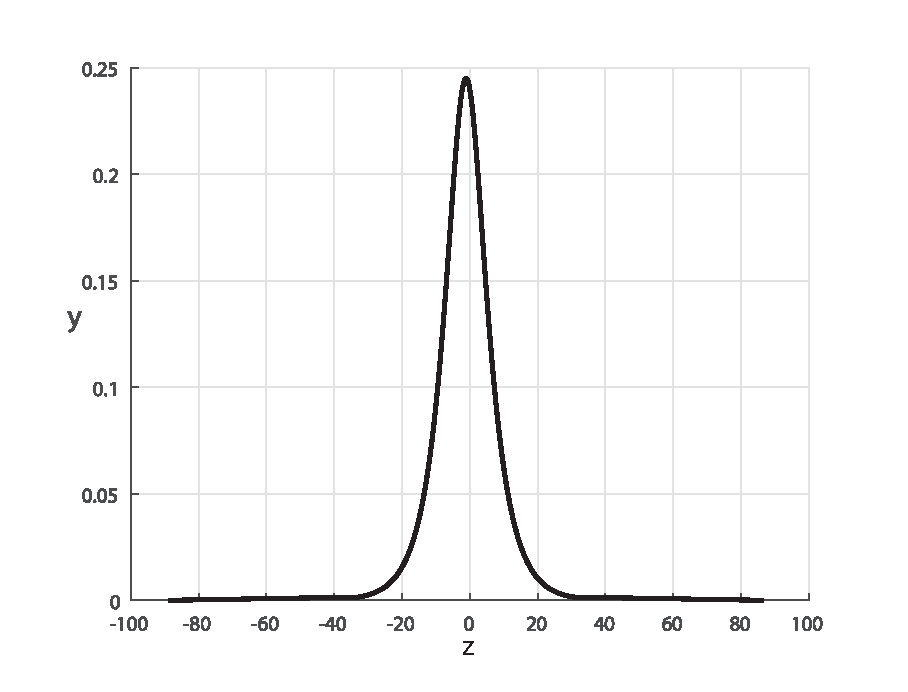
\includegraphics[width=0.5\linewidth]{Medvedev_fig4.eps}
		\caption{Профиль уединённой волны при \(k=1.6,\, M_{0}=-1.48,\, M_{1}=6.16.\)}
		\label{fig8}
	\end{figure}
\subsection[Модификация метода Фурье для моделирования процессов, описываемых уравнением Шрёдингера с тремя нелинейностями]{Модификация метода Фурье для моделирования процессов, описываемых уравнением Шрёдингера с тремя нелинейностями}\label{ch220}
	Семейство обобщённых уравнений Шрёдингера может быть записано в виде:
	\begin{equation} \label{eq220-1}
		u_{t}=i\mathscr{L} [u]+i\mathscr{N}[u]u.
	\end{equation}
	К примеру, при \(\mathscr{L} [u] \equiv a u_{xx},  \,\,  \mathscr{N} [u] \equiv b_{1} |u|^2\) уравнение (\ref{eq220-1}) представляет из себя нелинейное уравнение Шрёдингера (\ref{eq1}).

	Для применения метода Фурье, объявим периодические граничные условия следующим образом:
	\begin{equation} \label{eq30}
		\begin{aligned}
			\begin{cases}
				u\left(-\frac{L}{2},t\right)=u\left(\frac{L}{2},t\right),\\
				\cfrac{\partial u}{\partial x}\left(-\frac{L}{2},t\right)=\cfrac{\partial u}{\partial x}\left(\frac{L}{2},t\right).
			\end{cases}
		\end{aligned}
	\end{equation}

	Предполагая \( x \in [-\frac{1}{2} L, \frac{1}{2} L]\), \( t \in [0, T]\), разделим интервал по переменной \(x\) на \(N\) одинаковых частей с шагом
	\begin{equation}
		h=\frac{L}{N}.
	\end{equation}

	Узлы координатной сетки определяются, как
	\begin{equation}
		x_{j}=jh, \quad j= -\frac{N}{2}, \ldots , \frac{N}{2}.
	\end{equation}

	Пусть \(\boldsymbol{U}^{m}\) - сеточная аппроксимация решения на \(m\)-ном временном слое, и \(\boldsymbol{V}^{m}\) - промежуточное решение. В таком случае, начальные условия задаются в \(\boldsymbol{U}^{0}\). В общем виде, схема расщепления может быть записана следующим образом \cite{Rad1}:
	\begin{equation}\label{eq34}
		\boldsymbol{U}^{m+1}=e^{i\tau\mathscr{L}}\boldsymbol{V}^m,
	\end{equation}
	где
	\begin{equation}\label{eq33}
		\boldsymbol{V}^m=e^{i\tau\mathscr{N}[\boldsymbol{U}^m]}\boldsymbol{U}^m.
	\end{equation}

	Применяя метод Фурье, используем дискретное преобразование Фурье для сеточной функции \(\boldsymbol{V}^m\) для определения решения на следующем временном слое:
	\begin{equation} 
		\hat{\boldsymbol{V}}^m=\frac{h}{L}\exp\left(-i \boldsymbol{\mu} \boldsymbol{x}^{T}\right)\cdot \boldsymbol{V}^{m},
	\end{equation}
	где \(\hat{\boldsymbol{V}}^m\) - вектор коэффициентов Фурье, \(\boldsymbol{\mu}=\left(\mu_{-N/2},\ldots,\mu_{N/2-1}\right)^{T}\) - вектор частот преобразования \(\mu_{n}=\frac{2\pi n}{L}\), \(\boldsymbol{x}=\left(x_{-N/2},\ldots,x_{N/2-1}\right)^{T}\) - координаты точек сетки.

	Далее воспользуемся соотношением между \(\hat{\boldsymbol{U}}^{m+1}\) и \(\hat{\boldsymbol{V}}^{m}\),
	\begin{equation} \label{eq46}
		\hat{\boldsymbol{U}}^{m+1}=\exp\left(-i \left(\boldsymbol{\mu}\circ \boldsymbol{\mu}\right) \tau\right)\circ \hat{\boldsymbol{V}}^{m},
	\end{equation}
	которое вытекает из уравнения (\ref{eq34}) после подстановки в него вместо \(\boldsymbol{U}^{m+1}\) и \(\boldsymbol{V}^{m}\) соответствующих рядов Фурье. Под \(x\circ y\) понимается произведение по Адамару.

	Решение на следующем временном слое восстанавливается с помощью обратного преобразования Фурье, используя (\ref{eq46}):
	\begin{equation}
		\boldsymbol{U}^{m+1}=\exp\left(i \boldsymbol{\mu} \boldsymbol{x}^{T}\right)\cdot \hat{\boldsymbol{U}}^{m+1}.
	\end{equation}

	Модифицируя метод применительно к уравнению (\ref{eq200-4}), запишем операторы \(\mathscr{L} [u]\) и \(\mathscr{N}[u]\) в виде:
	\begin{equation}
		\begin{cases}
			\mathscr{L} [u] \equiv u_{xx},\\
			\mathscr{N} [u] \equiv |u|^2+ \varepsilon_{2}|u|^4+ \varepsilon_{3}|u|^6.
		\end{cases}
	\end{equation}

	Упрощённая блок-схема программного кода для численного решения проблемы распространения оптических импульсов при периодических граничных условиях представлена на Рис. \ref{fig2}.
	\begin{figure}[H]
		\begin{center}
			\begin{minipage}[h]{0.49\linewidth} %% color here
				\includegraphics[width=1\linewidth]{Medvedev_fig2.png}
			\end{minipage}
			\hfill
			\begin{minipage}[h]{0.49\linewidth}
				\includegraphics[width=0.75\linewidth]{Medvedev_fig3.png}
			\end{minipage}
		\end{center}
		\caption{Блок-схема программы, моделирующей процессы распространения импульсов с помощью метода Фурье.}
		\label{fig2}
	\end{figure}
\section{Численный анализ}\label{ch300}
\subsection{Применение метода Фурье для моделирования процесса распространения уединённой волны, описываемой уравнением Шрёдингера с тремя нелинейностями}\label{ch310}
	Рассмотрим процесс распространения уединённой волны (\ref{eq24}) уравнения (\ref{eq200-4}). Произведём расчёт при помощи схемы, описанной в разделе \ref{ch220} для определённых параметров \(M_{0}\) и \(M_{1}\), удовлетворяющих условиям (\ref{eq27}). Параметры \(\varepsilon_{1}\),\,\(\varepsilon_{2}\),\,\(\omega\) и \(\mu\) определяются формулами (\ref{eq19}). Результат моделирования представлен на Рис.\ref{fig10}. Аналитический и численно полученный профили в момент \(t=16\) изображены на Рис. \ref{fig10b}.

	\begin{figure}[H]
		\begin{center}
			\begin{minipage}[h]{0.48\linewidth} %% color here
				\includegraphics[width=1\linewidth]{Medvedev_fig5.eps}
				\subcaption{Модуль численного решения}
				\label{fig10a}
			\end{minipage}
			\hfill
			\begin{minipage}[h]{0.48\linewidth}
				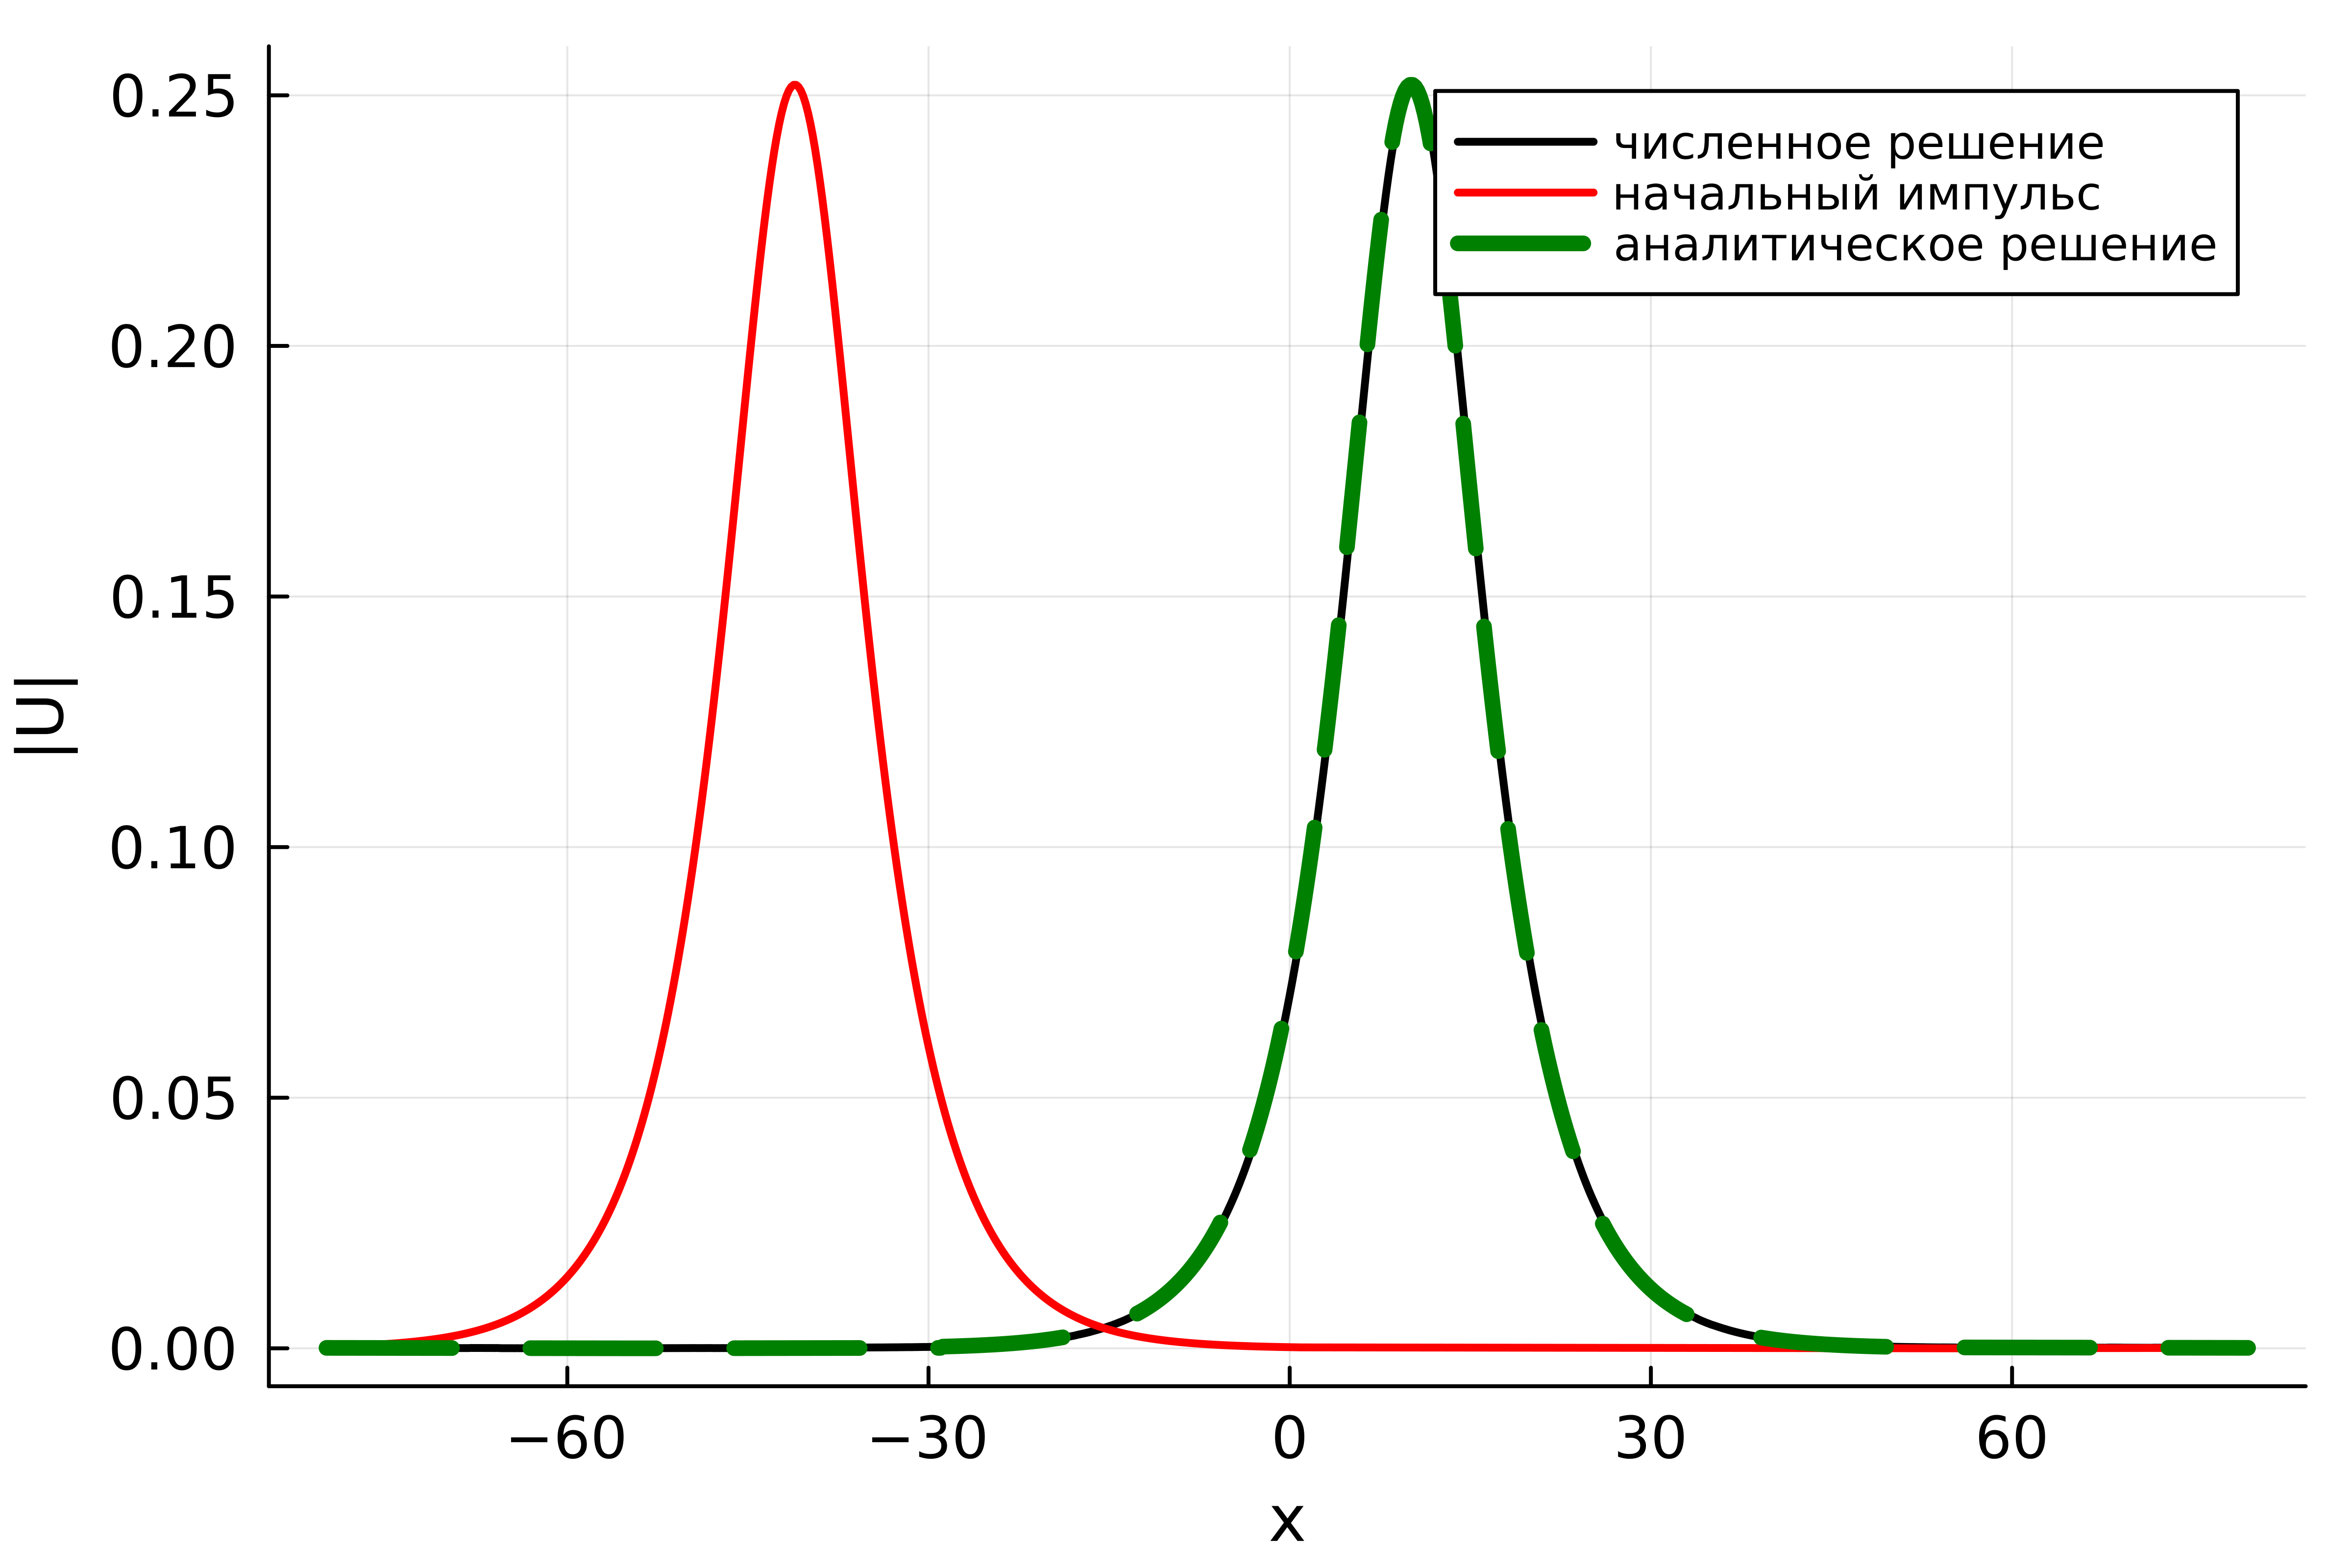
\includegraphics[width=1\linewidth]{Medvedev_fig6.eps}
				\subcaption{Модули решений при t=16}
				\label{fig10b}
			\end{minipage}
		\end{center}
		\caption{Распространение уединённой волны (\ref{eq24}) \\
		при параметрах
		\(L=120,\, T=16,\, h=0.2,\, \tau=0.04\), 
		\(z_{0}=-20,\,k=1.6,\, M_{0}=-1.48,\, M_{1}=6.16\).}
		\label{fig10}
	\end{figure}
	Относительная погрешность расчета при заданных параметрах не превышает 0.08.\%. Зависимость относительной погрешности от времени проиллюстрирована на Рис. \ref{fig11a}.

	\begin{figure}[H]
		\begin{center}
			\begin{minipage}[h]{0.48\linewidth} %% color here
				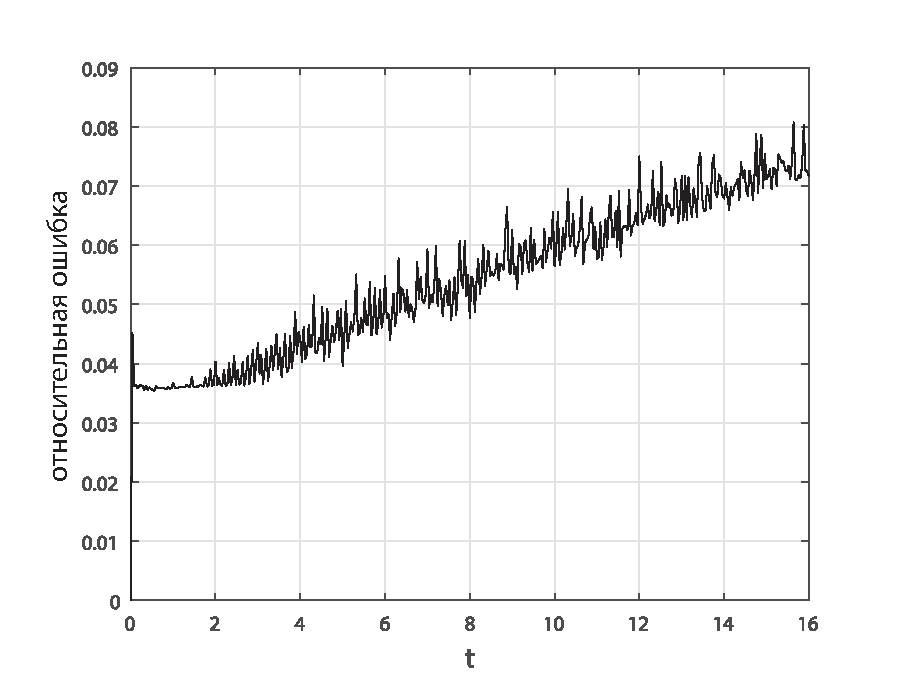
\includegraphics[width=1\linewidth]{Medvedev_fig7.eps}
				\subcaption{Относительная ошибка в зависимости от времени при \(h=0.2,\, \tau=0.04\)} 
				\label{fig11a}
			\end{minipage}
			\hfill
			\begin{minipage}[h]{0.48\linewidth}
				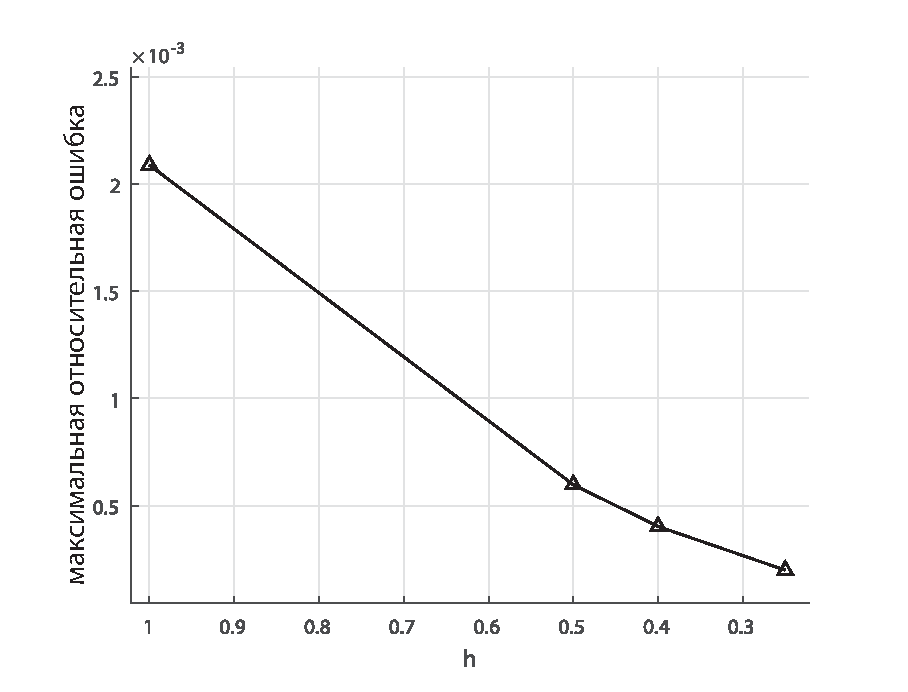
\includegraphics[width=1\linewidth]{Medvedev_fig15.eps}
				\subcaption{Максимальная относительная ошибка в зависимости от шага сетки \(h\)}
				\label{fig11b}
			\end{minipage}
		\end{center}
		\caption{Численные результаты при параметрах
		\(L=120,\, T=16\), 
		\(M_{0}=-1.48,\, M_{1}=6.16\).}
		\label{fig11}
	\end{figure}
	Сеточная сходимость достигнута (Рис. \ref{fig11b}), аналитическое решение совпало с численным. Следовательно, численная схема реализована корректно, и аналитическое решение, построенное в разделе \ref{ch210}, обладает солитонными свойствами.
\subsection{Взаимодействие солитона с возмущением в начальных условиях}\label{ch320}
	Проведём моделирование распространения импульса при возмущении в начальных условиях. Внесём в начальное условие, соответствующее решению (\ref{eq24}) уравнения (\ref{eq200-4}) возмущение следующим образом:
	\begin{equation} \label{eq52}
		u(x,0)=y\left(\xi\left(x\right)\right)\cdot e^{i(kx-\theta_{0})}+Ae^{-\nu(x-x_{0})^{2}}.
	\end{equation}
	Соответствующие численные результаты изображены на Рис. \ref{fig17}.
	\begin{figure}[H] %% color here
		\begin{center}
			\begin{minipage}[h]{0.48\linewidth}
				\includegraphics[width=1\linewidth]{Medvedev_fig8.eps}
				\subcaption{Модуль начального условия (\ref{eq52})}
			\end{minipage}
			\hfill
			\begin{minipage}[h]{0.48\linewidth}
				\includegraphics[width=1\linewidth]{Medvedev_fig9.eps}
				\subcaption{Модуль численного решения}
			\end{minipage}
		\end{center}
		\caption{Численные результаты при параметрах \(M_{0}=-3,\,M_{1}=12.34,\, k=3,\, \xi_{0}=0,\,z_{0}=-80,\, \theta_{0}=0\), \\
		\(L=300,\, T=32,\, h=0.25,\, \tau=0.625,\,A=0.2,\,\nu=0.06,\, x_{0}=25\).}
		\label{fig17}
	\end{figure}
	Проведённое моделирование позволяет сделать вывод, что солитон, заданный рассмотренными параметрами \(M_{0}=-3,\,M_{1}=12,34\), взаимодействует с заданным возмущением, не распадаясь и не теряя способности к распространению. Профиль пульса восстанавливается после взаимодействия.

	Также установлено, что солитон (\ref{eq200-4}) устойчив при распространении в среде со случайным шумом следующего вида:
	\begin{equation} \label{eq522}
		u(x,0)=y\left(\xi\left(x\right)\right)\cdot e^{i(kx-\theta_{0})}+A\cdot rand(x).
	\end{equation}
	Результаты моделирования проиллюстрированы на Рис. \ref{fig172}.	
	\begin{figure}[H] %% color here
		\begin{center}
			\begin{minipage}[h]{0.48\linewidth}
				\includegraphics[width=1\linewidth]{Medvedev_fig16.eps}
				\subcaption{Модуль численного решения}
			\end{minipage}
			\hfill
			\begin{minipage}[h]{0.48\linewidth}
				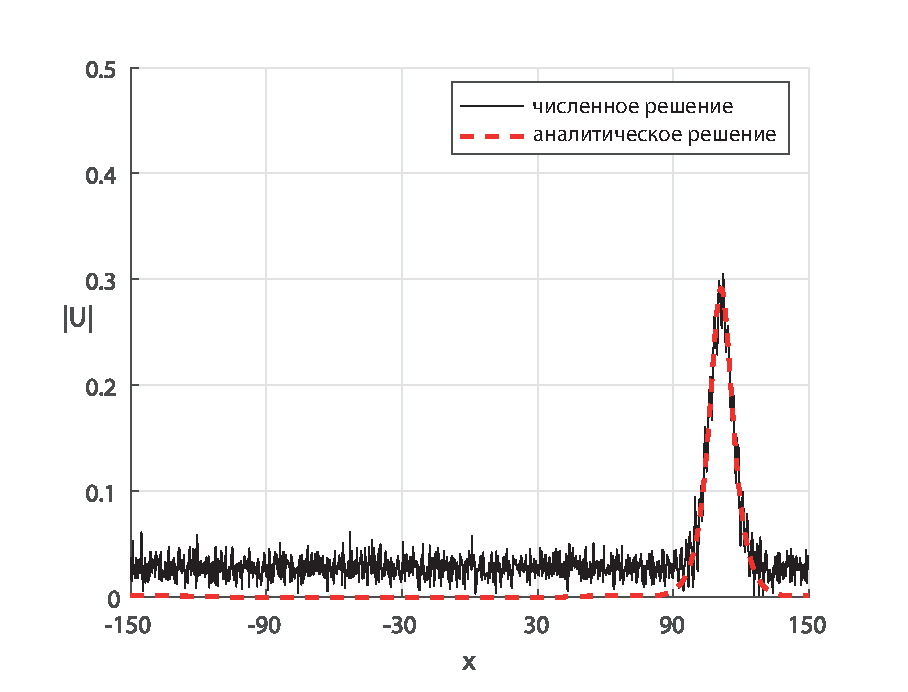
\includegraphics[width=1\linewidth]{Medvedev_fig17.eps}
				\subcaption{Профили решений при t=32}
			\end{minipage}
		\end{center}
		\caption{Численные результаты при параметрах \(M_{0}=-3,\,M_{1}=12.34,\, k=3,\, \xi_{0}=0,\,z_{0}=-80,\, \theta_{0}=0\), \\
		\(L=300,\, T=32,\, h=0.25,\, \tau=0.0625,\,A=0.05\).}
		\label{fig172}
	\end{figure}

	Моделирования, представленные в данном разделе, подтверждают стабильность солитонов, полученных в разделе \ref{ch210}.
\subsection{Анализ влияния высших степеней нелинейности на распространение уединённой волны}\label{ch330}
	При решении физических задач классическое НУШ обобщается путём добавления в уравнение некоторых выражений, учитывающих определённые физические факторы. Поскольку реальные физические процессы могут протекать по более сложным законам, не всегда возможно заранее предугадать и учесть все необходимые уточняющие члены. В этом разделе мы исследуем влияние дополнительных нелинейных членов на решения НУШ.
	При \(\varepsilon_{2}=0,\,\varepsilon_{3}=0\), уравнение (\ref{eq200-4}) является НУШ:
	\begin{equation}\label{e6}
		iu_{t}+u_{xx}+|u|^2 u=0.
	\end{equation}
	Задача Коши для уравнения (\ref{e6}) решается методом обратной задачи рассеяния. Его решение в виде уединенной волны представлено в работе \cite{Rad3} и имеет вид:
	\begin{equation} \label{eq48}
		u(x,t)=\frac{4(\omega-k^{2})}{2 (\omega-k^{2}) e^{-\left(x-c_{0}t-z_{0}\right)\sqrt{(\omega-k^{2})}}+e^{\left(x-c_{0}t-z_{0}\right)\sqrt{(\omega-k^{2})}}}\cdot e^{i(kx-\omega t-\theta_{0})},
	\end{equation}
	где \(c_{0}=2k\) и \( k,\, \omega,\, z_{0},\, \theta_{0}\) - произвольные константы.
	Начальное условие, относящееся к решению (\ref{eq48}) имеет вид:
	\begin{equation}\label{eq55}
		u(x,0)=\frac{4\,(\omega-k^{2})}{2 (\omega-k^{2}) e^{-(x-z_{0})\sqrt{(\omega-k^{2})}}+e^{(x-z_{0})\sqrt{(\omega-k^{2})}}}\cdot e^{i(kx-\theta_{0})}
	\end{equation}

	При \(\varepsilon_{3}=0\), решение уравнения (\ref{eq200-4}) было также найдено в следующем виде:
	\begin{equation}\label{e7}
		u(x,t)=\left(\frac{4\,\mu\, e^{\sqrt{\mu}\,(x-2kt-z_{0})}}{1+4\, e^{\sqrt{\mu}\,(x-2kt-z_{0})}+(4+4\, \mu\, \nu) \,e^{2\sqrt{\mu}\,(x-2kt-z_{0})}}\right)^{\frac{1}{2}}\cdot e^{i(kx-\omega t-\theta_{0})},
	\end{equation}
	где \(\mu=4(\omega-k^{2})\), \(\nu=\cfrac{4 \varepsilon_{2}}{3}\) и \( k,\, \omega,\, z_{0},\, \theta_{0}\) - произвольные константы. Заметим, что при \(\varepsilon_{2}=0\) решение (\ref{e7}) совпадает с решением (\ref{eq48}).

	Исследуем влияние нелинейных выражений на распространение уединённой волны (\ref{eq55}) в рамках модели, описываемой уравнением (\ref{eq200-4}).

	При \(\varepsilon_{2}=0,\,\varepsilon_{3}=0\) уединенная волна (\ref{eq48}) является точным решением уравнения (\ref{eq200-4}). Численное решение для начального условия (\ref{eq55}) совпадает с аналитическим.

	В случае введения нелинейного члена при \(\varepsilon_{2}\ne 0\), импульс претерпевает изменения в процессе распространения. Поскольку начальное условие (\ref{eq55}) не удовлетворяет уравнению модели (\ref{eq200-4}), солитонные свойства импульса перестают выполняться, и его форма постепенно изменяется. Излучение энергии при граничных периодических условиях нарушает изначальное предположение об уединённости импульса. Для восстановления справедливости данного предположения, в процесс расчёта введена процедура фильтрации излучения в численном решении.

	Обнаружено, что форма импульса (\ref{eq55}) постепенно становится устойчивой. Установлено, что для установившегося импульса существует солитон вида (\ref{e7}), совпадающий по форме. Данное наблюдение позволяет заключить, что исходный импульс под влиянием нелинейных выражений в модели преобразуется в импульс, совпадающий с аналитическим решением (\ref{e7}) уравнения (\ref{eq200-4}) при \(\varepsilon_{3}=0\). Результаты моделирования проиллюстрированы на Рис. \ref{fig21_1} и \ref{fig21_2}.
	\begin{figure}[H] %% color here
		\begin{center}
			\begin{minipage}[h]{0.48\linewidth}
				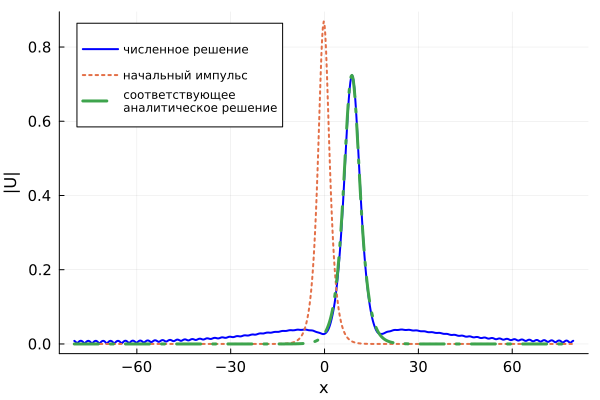
\includegraphics[width=1\linewidth]{Medvedev_fig10.png}
				\subcaption{Профиль решения при t=30}
			\end{minipage}
			\hfill
			\begin{minipage}[h]{0.48\linewidth}
				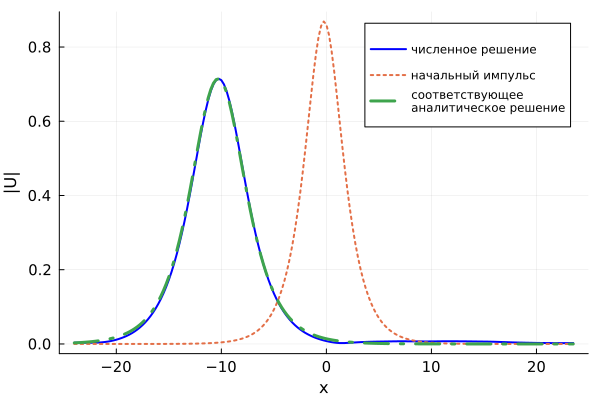
\includegraphics[width=1\linewidth]{Medvedev_fig11.png}
				\subcaption{Профиль решения при t=500}
			\end{minipage}
		\end{center}
		\caption{Численные результаты распространения импульса (\ref{eq55}) при
		\(L=160,\, T=500,\, h=0.25,\, \tau=0.0625,\)
		\(\varepsilon_{2}=-0.5,\,\varepsilon_{3}=0,\, \omega=0.4,\, k=0.15\).}
		\label{fig21_1}
	\end{figure}

	Относительная ошибка между аналитическим решением (\ref{e7}) и полученным численным решением от времени представлена на Рис. \ref{fig21_2a}.
	\begin{figure}[H]
		\begin{center}
			\begin{minipage}[h]{0.48\linewidth}
				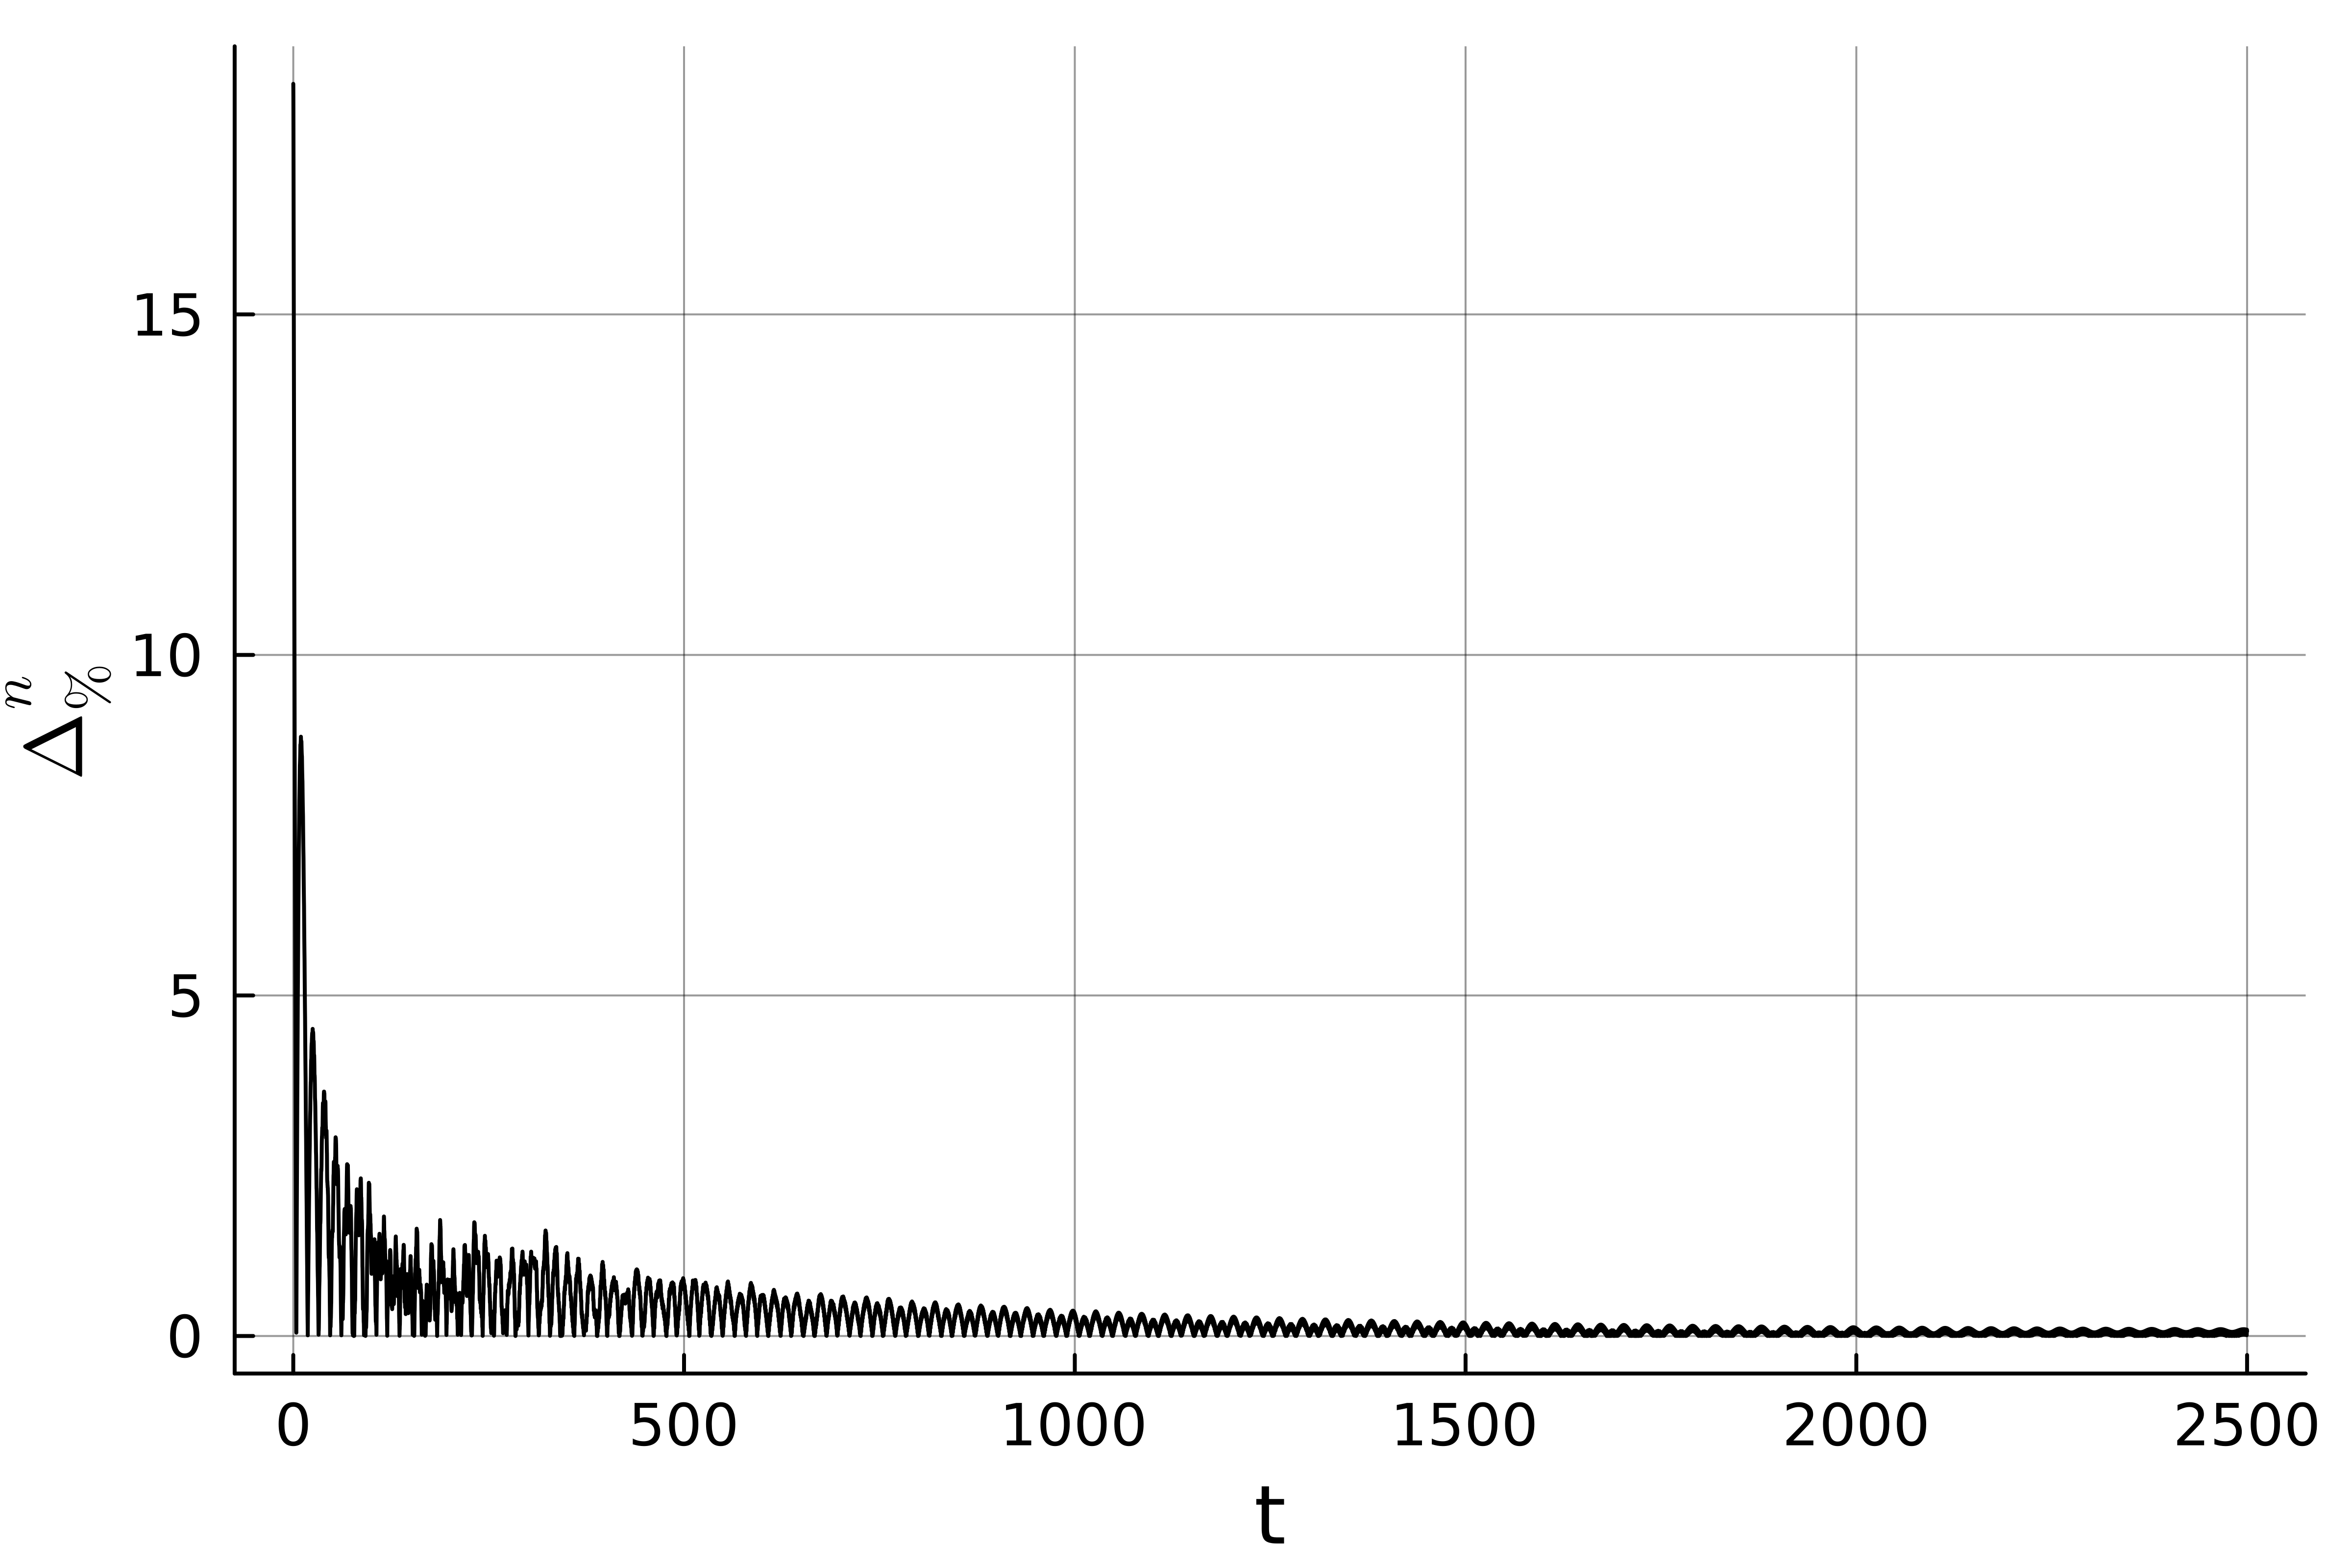
\includegraphics[width=1\linewidth]{Medvedev_fig18.png}
				\subcaption{Относительная ошибка в зависимости от времени}
				\label{fig21_2a}
			\end{minipage}
			\hfill
			\begin{minipage}[h]{0.48\linewidth}
				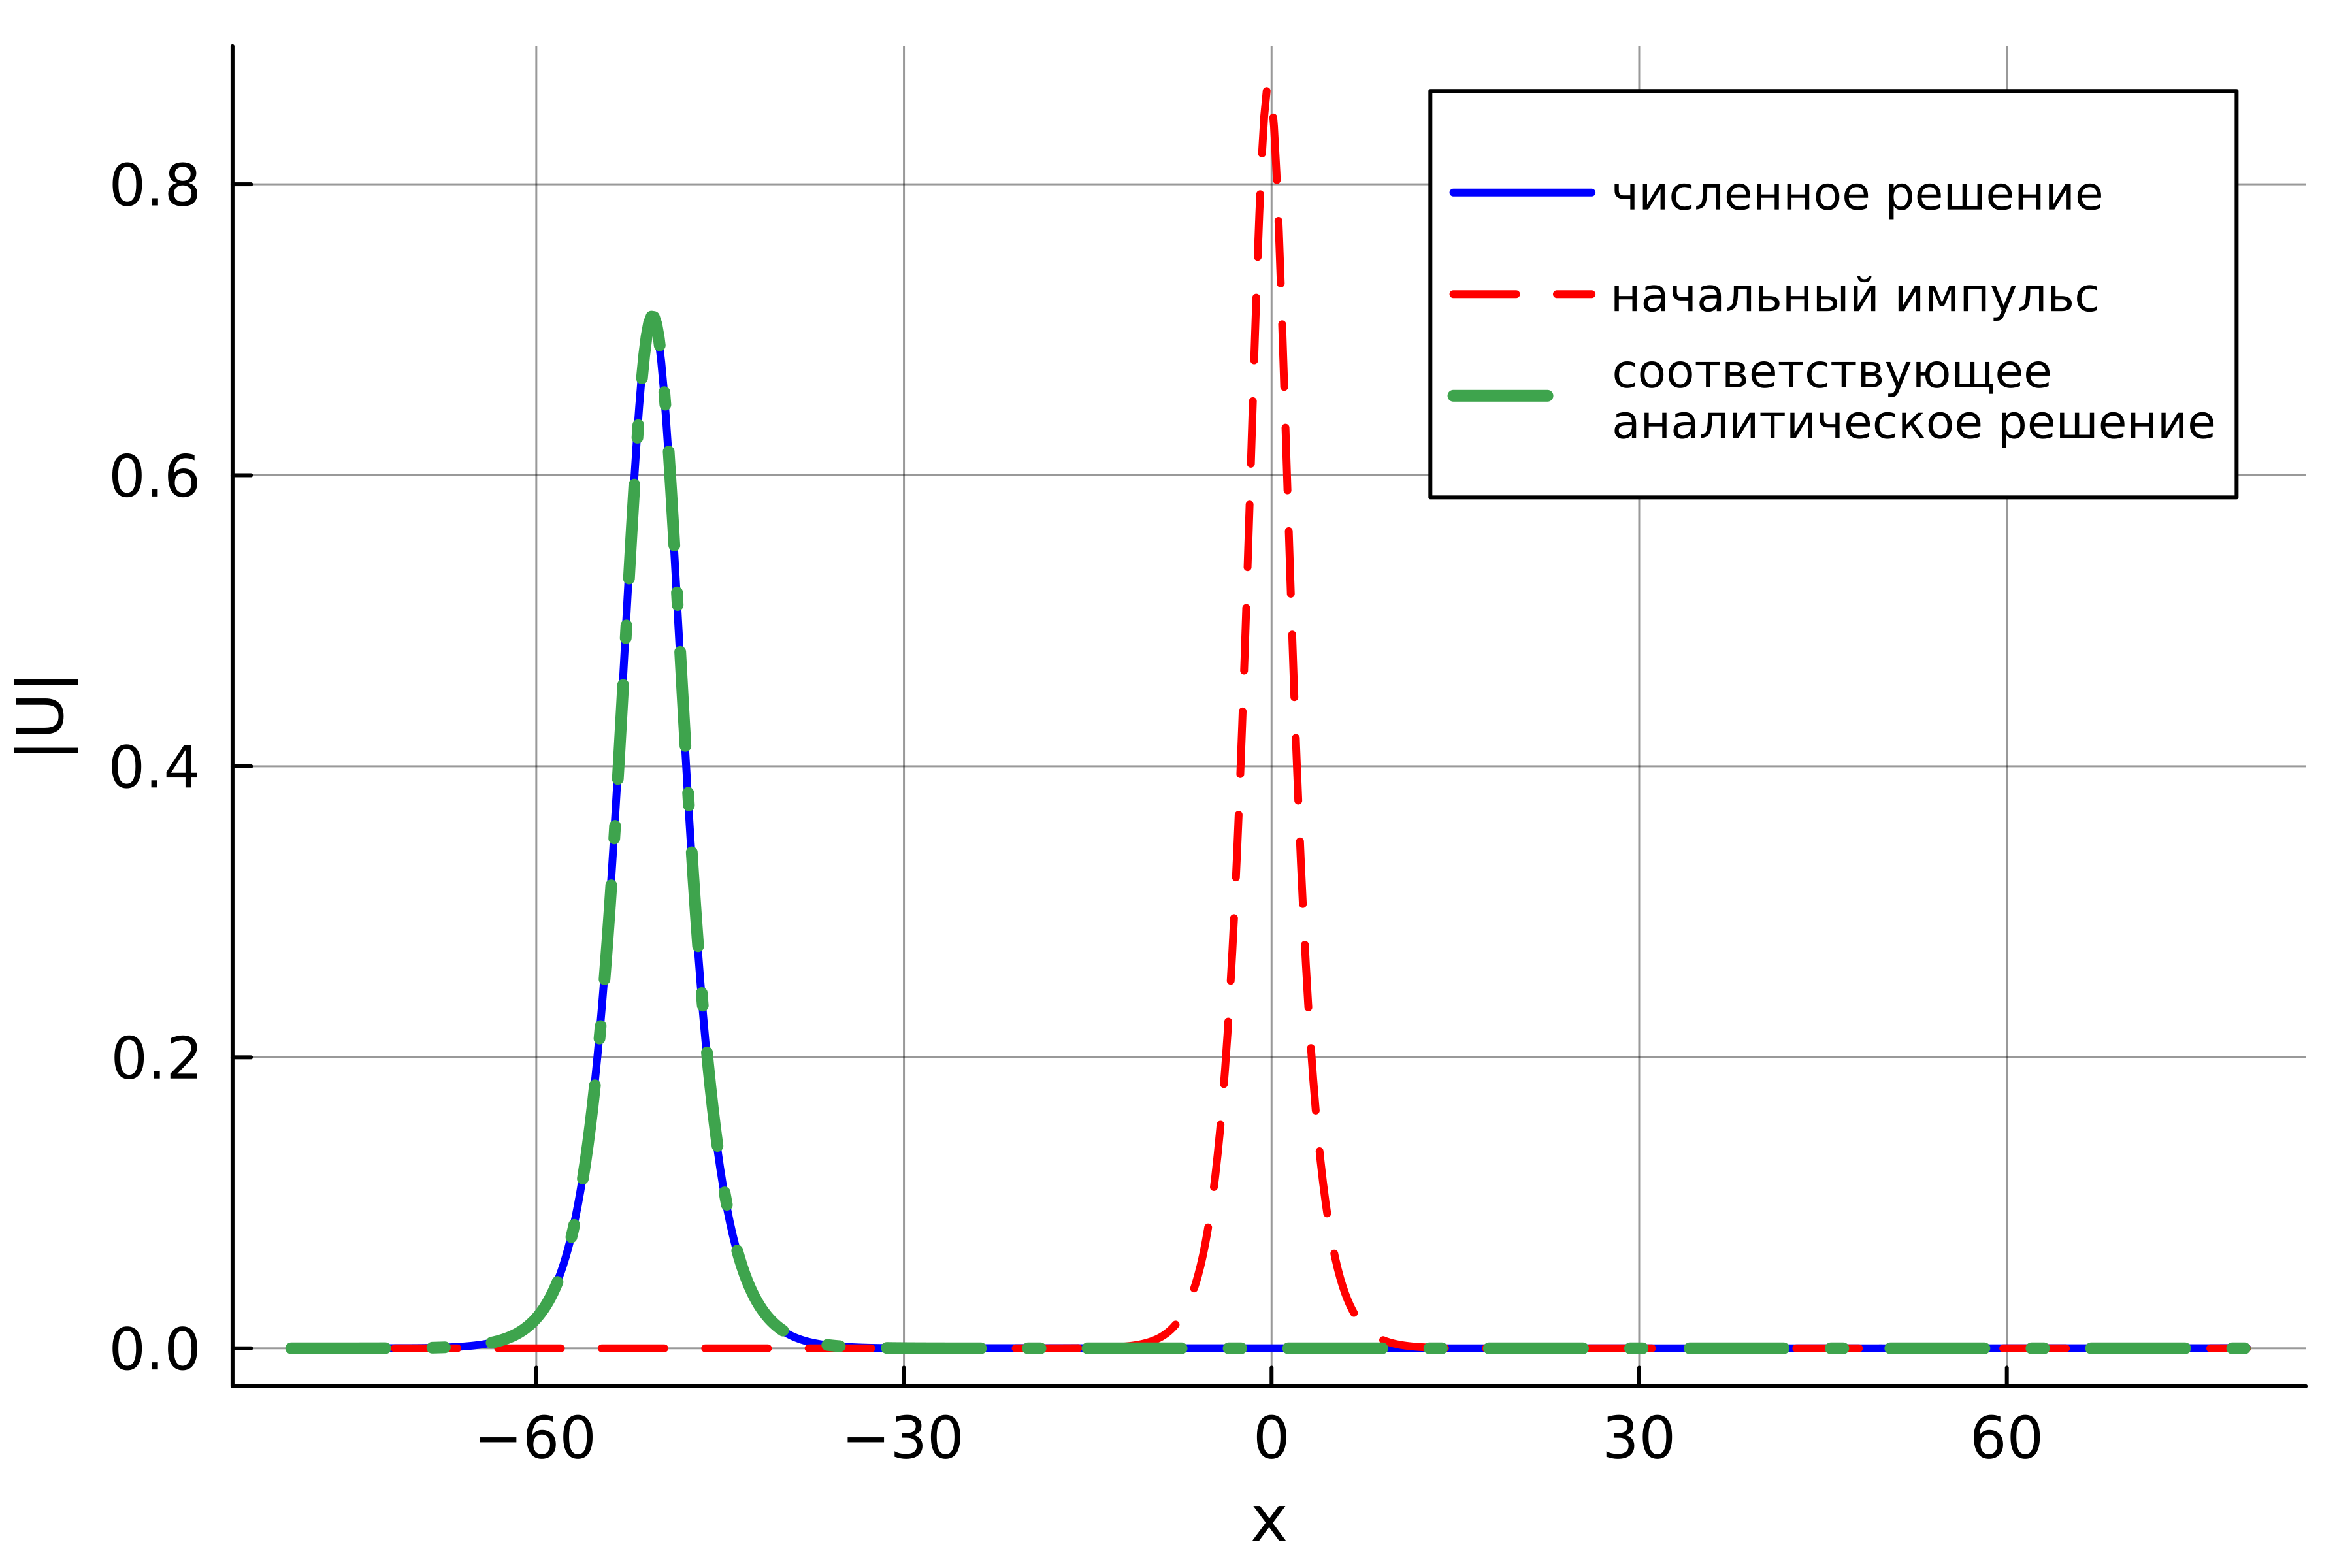
\includegraphics[width=1\linewidth]{Medvedev_fig19.png}
				\subcaption{Профиль решения при t=2500}
				\label{fig21_2b}
			\end{minipage}
		\end{center}
		\caption{Численные результаты распространения импульса (\ref{eq55}) при
		\(L=160,\, T=500,\, h=0.25,\, \tau=0.0625,\)
		\(\varepsilon_{2}=-0.5,\,\varepsilon_{3}=0,\, \omega=0.4,\, k=0.15\).}
		\label{fig21_2}
	\end{figure}

	Рассмотрим добавление в модель нелинейного члена седьмой степени при \(\varepsilon_{3}\ne0\). При этом форма импульса также изменяется. Установлено влияние знака \(\varepsilon_{3}\) на затухание колебаний. При \(\varepsilon _{3}<0\) амплитуда результирующего импульса уменьшается относительно исходного. При \(\varepsilon _{3}>0\) амплитуда полученного импульса возрастает. Колебания устанавливаются тем раньше по времени моделирования, чем меньше значение \(\varepsilon_{3}\). Зависимости амплитуды импульса от времени в зависимости от параметров возмущений проиллюстрированы на Рис. \ref{fig48}, где \(\delta\) — относительная амплитуда колебаний в конце временного промежутка моделирования.
	\begin{figure}[H] %% color here
		\begin{minipage}[h]{1\linewidth}
			\includegraphics[width=1\linewidth]{Medvedev_fig12.eps}
			\subcaption{\(\varepsilon_{2}=-0.5,\,\varepsilon_{3}=0\)}
			\includegraphics[width=1\linewidth]{Medvedev_fig13.eps}
			\subcaption{\(\varepsilon_{2}=-0.5,\,\varepsilon_{3}=-0.25\)}
			\includegraphics[width=1\linewidth]{Medvedev_fig14.eps}
			\subcaption{\(\varepsilon_{2}=-0.5,\,\varepsilon_{3}=0.25\)}
		\end{minipage}
		\caption{Зависимость амплитуды импульса (\ref{eq55}) при распространении .
		\(L=200,\, T=5000,\, h=0.25,\, \tau=0.0625,\, \omega=0.2,\, k=0.707\).}
		\label{fig48}
	\end{figure}

	Результаты, представленные в данном разделе, позволяют сделать вывод, что уединенные волны НУШ при распространении в среде с высшими нелинейными членами при определённых параметрах преобразуются в устойчивые солитоны обобщенной неинтегрируемой модели. Этот переход сопровождается излучением энергии. Обнаружено, что добавление нелинейного члена 7-й степени влияет на скорость преобразования исходного импульса в устойчивый, и на форму итогового импульса. Данное влияние определяется величиной и знаком параметра \(\varepsilon_{3}\).
\subsection{Столкновения солитонов в присутствии высших степеней нелинейности}\label{ch340}
	Известно, что решения интегрируемого нелинейного уравнения Шрёдингера взаимодействуют упруго, т.е. без обмена импульсом и энергией. При нарушении интегрируемости системы внешними возмущениями солитонные столкновения становятся неупругими. В этом разделе мы исследуем столкновения солитонов НУШ в среде, описываемой возмущённым уравнением (\ref{eq200-4}).

	Рассмотрим столкновения двух солитонов вида (\ref{eq55}) с заданными параметрами \(k_{1},\,k_{2},\,\omega_{1},\,\omega_{2},\,z_{0,1},\,z_{0,2},\,\theta_{0,1},\,\theta_{0,2}\). Значения параметров \(\varepsilon_{2}\) и \(\varepsilon_{3}\) в данном случае влияют на интенсивность обмена импульсом и энергией. Обнаружено, что итоговый характер взаимодействия солитонов зависит также от разности фаз в момент столкновения \(\Delta \theta=\theta_{0,1}-\theta_{0,2}\).

	Результаты моделирования для \(k_{1}=-k_{2},\,\omega_{1}=\omega_{2},\,z_{0,1}=-z_{0,2},\,\theta_{0,1}=\theta_{0,2}+\Delta \theta\) проиллюстрированы на Рис. \ref{fig50} и Рис. \ref{fig51}.

	\begin{figure}[H]
		\begin{minipage}[h]{0.32\linewidth}
			\includegraphics[width=1\linewidth]{Medvedev_fig20.eps}
			\subcaption{\(\Delta \theta=0,\)\\\( \varepsilon_{2}=0.2,\,\varepsilon_{3}=-0.1\)}
		\end{minipage}
		\begin{minipage}[h]{0.32\linewidth}
			\includegraphics[width=1\linewidth]{Medvedev_fig26.eps}
			\subcaption{\(\Delta \theta=\frac{\pi}{2},\)\\\( \varepsilon_{2}=0.2,\,\varepsilon_{3}=-0.1\)}
		\end{minipage}
		\begin{minipage}[h]{0.32\linewidth}
			\includegraphics[width=1\linewidth]{Medvedev_fig32.eps}
			\subcaption{\(\Delta \theta=\pi,\)\\\( \varepsilon_{2}=0.2,\,\varepsilon_{3}=-0.1\)}
		\end{minipage}

		\begin{minipage}[h]{0.32\linewidth}
			\includegraphics[width=1\linewidth]{Medvedev_fig22.eps}
			\subcaption{\(\Delta \theta=0,\)\\\( \varepsilon_{2}=0.4,\,\varepsilon_{3}=-0.2\)}
		\end{minipage}
		\begin{minipage}[h]{0.32\linewidth}
			\includegraphics[width=1\linewidth]{Medvedev_fig28.eps}
			\subcaption{\(\Delta \theta=\frac{\pi}{2},\)\\\( \varepsilon_{2}=0.4,\,\varepsilon_{3}=-0.2\)}
		\end{minipage}
		\begin{minipage}[h]{0.32\linewidth}
			\includegraphics[width=1\linewidth]{Medvedev_fig34.eps}
			\subcaption{\(\Delta \theta=\pi,\)\\\( \varepsilon_{2}=0.4,\,\varepsilon_{3}=-0.2\)}
		\end{minipage}

		\begin{minipage}[h]{0.32\linewidth}
			\includegraphics[width=1\linewidth]{Medvedev_fig24.eps}
			\subcaption{\(\Delta \theta=0,\)\\\( \varepsilon_{2}=0.6,\,\varepsilon_{3}=-0.3\)}
		\end{minipage}
		\begin{minipage}[h]{0.32\linewidth}
			\includegraphics[width=1\linewidth]{Medvedev_fig30.eps}
			\subcaption{\(\Delta \theta=\frac{\pi}{2},\)\\\( \varepsilon_{2}=0.6,\,\varepsilon_{3}=-0.3\)}
		\end{minipage}
		\begin{minipage}[h]{0.32\linewidth}
			\includegraphics[width=1\linewidth]{Medvedev_fig36.eps}
			\subcaption{\(\Delta \theta=\pi,\)\\\( \varepsilon_{2}=0.6,\,\varepsilon_{3}=-0.3\)}
		\end{minipage}
		\caption{Модуль численного решения при моделировании солитонных столкновений для \(k_{1}=-k_{2}=0.7,\,\omega_{1}=\omega_{2}=0\).}
		\label{fig50}
	\end{figure}

	\begin{figure}[H]
		\begin{minipage}[h]{0.32\linewidth}
			\includegraphics[width=1\linewidth]{Medvedev_fig21.eps}
			\subcaption{\(\Delta \theta=0,\)\\\( \varepsilon_{2}=0.2,\,\varepsilon_{3}=-0.1\)}
		\end{minipage}
		\begin{minipage}[h]{0.32\linewidth}
			\includegraphics[width=1\linewidth]{Medvedev_fig27.eps}
			\subcaption{\(\Delta \theta=\frac{\pi}{2},\)\\\( \varepsilon_{2}=0.2,\,\varepsilon_{3}=-0.1\)}
		\end{minipage}
		\begin{minipage}[h]{0.32\linewidth}
			\includegraphics[width=1\linewidth]{Medvedev_fig33.eps}
			\subcaption{\(\Delta \theta=\pi,\)\\\( \varepsilon_{2}=0.2,\,\varepsilon_{3}=-0.1\)}
		\end{minipage}

		\begin{minipage}[h]{0.32\linewidth}
			\includegraphics[width=1\linewidth]{Medvedev_fig23.eps}
			\subcaption{\(\Delta \theta=0,\)\\\( \varepsilon_{2}=0.4,\,\varepsilon_{3}=-0.2\)}
		\end{minipage}
		\begin{minipage}[h]{0.32\linewidth}
			\includegraphics[width=1\linewidth]{Medvedev_fig29.eps}
			\subcaption{\(\Delta \theta=\frac{\pi}{2},\)\\\( \varepsilon_{2}=0.4,\,\varepsilon_{3}=-0.2\)}
		\end{minipage}
		\begin{minipage}[h]{0.32\linewidth}
			\includegraphics[width=1\linewidth]{Medvedev_fig35.eps}
			\subcaption{\(\Delta \theta=\pi,\)\\\( \varepsilon_{2}=0.4,\,\varepsilon_{3}=-0.2\)}
		\end{minipage}

		\begin{minipage}[h]{0.32\linewidth}
			\includegraphics[width=1\linewidth]{Medvedev_fig25.eps}
			\subcaption{\(\Delta \theta=0,\)\\\( \varepsilon_{2}=0.6,\,\varepsilon_{3}=-0.3\)}
		\end{minipage}
		\begin{minipage}[h]{0.32\linewidth}
			\includegraphics[width=1\linewidth]{Medvedev_fig31.eps}
			\subcaption{\(\Delta \theta=\frac{\pi}{2},\)\\\( \varepsilon_{2}=0.6,\,\varepsilon_{3}=-0.3\)}
		\end{minipage}
		\begin{minipage}[h]{0.32\linewidth}
			\includegraphics[width=1\linewidth]{Medvedev_fig37.eps}
			\subcaption{\(\Delta \theta=\pi,\)\\\( \varepsilon_{2}=0.6,\,\varepsilon_{3}=-0.3\)}
		\end{minipage}
		\caption{Действительная часть численного решения при моделировании солитонных столкновений для \(k_{1}=-k_{2}=0.7,\,\omega_{1}=\omega_{2}=0\).}
		\label{fig51}
	\end{figure}

	Результаты моделирования позволяют заключить, что столкновения солитонов НУШ в рамках математической модели, включающей нелинейные члены высшего порядка в зависимости от разности фаз в момент столкновения быть существенно неупругими. Вблизи \(\Delta \theta=\pi\) солитоны взаимодействуют наименее интенсивно. Когда разность фаз находится в окрестности нуля, происходит значительное энерговыделение. В этом случае существуют критические параметры возмущения, при которых два солитона сливаются в один стационарный. При параметре \(\Delta\theta\in (0,\,\pi)\) взаимодействие солитонов происходит с обменом энергией и импульсом. Помимо разности фаз, на определенный тип взаимодействия влияют значения параметров возмущения \(\varepsilon_{2}\) и \(\varepsilon_{3}\). Чем больше модуль коэффициента при соответствующей степени нелинейности, тем более выражен неупругий характер взаимодействия.
\section{Заключение}\label{ch400}
	В данной работе проведено численное моделирование процессов распространения импульсов в нелинейной оптической среде с периодическими граничными условиями, описываемой обобщённым уравнением Шрёдингера (\ref{eq120-1}) с нелинейными членами третьего, пятого и седьмого порядков. Получено аналитическое решение в виде уединенной волны (\ref{eq24}) и условия ее существования. Представлена модификация метода Фурье для численного решения поставленной задачи. С численной точки зрения исследован процесс распространения аналитически полученного солитонного решения обобщённой модели. Проведено моделирование взаимодействия оптического солитона уравнения (\ref{eq120-1}) с возмущением в начальных данных. Смоделировано распространение оптического импульса в среде со случайным шумом. Проанализировано влияние высших степеней нелинейности в математической модели на распространение уединенных волн нелинейного уравнения Шрёдингера. Проведено моделирование процессов столкновения солитонов в условиях наличия высших нелинейных членов.

	Следующие результаты получены в результате исследования:
	\begin{enumerate}
	\setlength\itemsep{1em}
		\item Уединённые волны уравнения Шрёдингера с нелинейными членами третьей, пятой и седьмой степеней распространяются устойчиво.
		\item Оптические солитоны уравнения Шрёдингера с нелинейными членами третьей, пятой и седьмой степеней не распадаются при возмущениями начальных условий или при распространении в условиях случайного шума.
		\item При распространении в оптической среде, описываемой математической моделью с нелинейными членами более высокого порядка солитоны НУШ преобразуются в солитоны, удовлетворяющие обобщённому уравнению. 
		\item В условиях наличия нелинейных членов высшего порядка столкновения солитонов НУШ происходят значительно неупруго. При определённых параметрах возможно образование стоячих волн.
	\end{enumerate}
\renewcommand\refname{Список литературы}
\begin{thebibliography}{9}
	\bibitem{Rad04} Bruce M Lake and Henry C Yuen and Harald Rungaldier and Warren E Ferguson, Nonlinear deep-water waves: theory and experiment. {P}art 2. {E}volution of a continuous wave train, \textit{Journal of Fluid Mechanics, Cambridge University Press, 1977. V. 83. No. 1 P. 49-74}.
	\bibitem{Rad05} Henry C. Yuen and Warren E. Ferguson, Relationship between {B}enjamin-{F}eir instability and recurrence in the nonlinear {S}chr\"{o}dinger equation, \textit{Physics of Fluids, 1978. V. 21. No. 8 P. 1275}.
	\bibitem{Rad9} Nikolay A. Kudryashov, On traveling wave solutions of the {K}undu-{E}ckhaus equation, \textit{Optik, 2020, V. 224. 165500.}.
	\bibitem{Rad015} Russell W. Kohl and Anjan Biswas and Mehmet Ekici and Qin Zhou and Salam Khan and Ali S. Alshomrani and Milivoj R.  Belic, Highly dispersive optical soliton perturbation with cubic-quintic-septic refractive index by semi-inverse variational principle, \textit{Optik, 2019, V. 199. 163322}.
	\bibitem{Rad017} Nikolay A. Kudryashov, Construction of nonlinear differential equations for description of propagation pulses in optical fiber, \textit{Optik, 2019, V. 192. 162964.}.
	\bibitem{Rad018} Nikolay A. Kudryashov, Solitary and periodic waves of the hierarchy for propagation pulse in optical fiber, \textit{Optik, 2019, V. 194. 163060.}.
	\bibitem{Rad019} Anjan Biswas and Mehmet Ekici and Abdullah Sonmezoglu and Milivoj R. Belic, Highly dispersive optical solitons with non-local nonlinearity by exp-function, \textit{Optik, 2019, V. 186. P. 288-292.}.
	\bibitem{Rad3} Nikolay A. Kudryashov, Method for finding optical solitons of generalized nonlinear {S}chr\"{o}dinger equations, \textit{Optik, 2022, V. 261. 169163.}.
	\bibitem{Rad02} Yuri Kivshar and Govind Agrawal, Optical Solitons: From Fibers to Photonic Crystals, \textit{Academic Press, 2003. P. 108.}.
	\bibitem{Rad4} Nikolai A. Kudryashov, Simplest equation method to look for exact solutions of nonlinear differential equations, \textit{Chaos, Solitons \& Fractals, 2005, V. 24. No. 5. P. 1217-1231.}.
	\bibitem{Rad1} J. A. C. Weideman and B. M. Herbst, Split-Step Methods for the Solution of the Nonlinear {S}chr\"{o}dinger Equation, \textit{SIAM Journal on Numerical Analysis, 1986, V. 23. No. 3. P. 485-507}.
\end{thebibliography}

\vskip 1.5em
\begin{center}
	{\textbf{Numerical study of soliton solutions of the cubic-quintic-septic nonlinear Schr\"{o}dinger equation} \par}\vskip 1em
	\textbf{V .A. Medvedev, N. A. Kudryashov}\\
	\emph{National Research Nuclear University MEPhI(Moscow Engineering Physics Institute), Moscow, 115409 Russia}\\
	\emph{email:  viktormedvedev12115551@gmail.com, nakudr@gmail.com}\\
\end{center}
\par

\bigskip
\textbf{Abstract} --
{The problem of pulse propagation described by the nonlinear Schr\"{o}dinger equation with non-Kerr nonlinearity of the third, fifth and seventh powers is considered. Optical solitons of the considered equation are found using simplest equations method and implicit functions method. The area of acceptable model parameters is illustrated. A modification of the split-step Fourier method is presented. Optical soliton propagation process is studied numerically. The process of the interaction of a soliton pulse with a disturbance in the initial condition is analyzed. The process of the soliton pulse propogation in a medium with a random noise simulated. The stability of optical solitons of the cubic-quintic-septic nonlinear Schr\"{o}dinger equation is proved. The influence of higher nonlinearity terms on the nonlinear Schr\"{o}dinger equation solitary waves is studied. The soliton collisions in the presence of higher nonlinear terms are simulated. It is shown that in the presence of higher nonlinear terms, the solitons interact inelastically upon collision.}\\

\textit{Keywords:} Cubic-quintic-septic nonlinear Schr\"{o}dinger equation, Split-step Fourier scheme, Optical soliton, Numerical modeling, Nonlinear optics, Nonlinear differential equations.

\renewcommand\refname{References}
\begin{thebibliography}{9}
	\bibitem{Rad04} Bruce M Lake and Henry C Yuen and Harald Rungaldier and Warren E Ferguson, Nonlinear deep-water waves: theory and experiment. {P}art 2. {E}volution of a continuous wave train, \textit{Journal of Fluid Mechanics, Cambridge University Press, 1977. V. 83. No. 1 P. 49-74}.
	\bibitem{Rad05} Henry C. Yuen and Warren E. Ferguson, Relationship between {B}enjamin-{F}eir instability and recurrence in the nonlinear {S}chr\"{o}dinger equation, \textit{Physics of Fluids, 1978. V. 21. No. 8 P. 1275}.
	\bibitem{Rad9} Nikolay A. Kudryashov, On traveling wave solutions of the {K}undu-{E}ckhaus equation, \textit{Optik, 2020, V. 224. 165500.}.
	\bibitem{Rad015} Russell W. Kohl and Anjan Biswas and Mehmet Ekici and Qin Zhou and Salam Khan and Ali S. Alshomrani and Milivoj R.  Belic, Highly dispersive optical soliton perturbation with cubic-quintic-septic refractive index by semi-inverse variational principle, \textit{Optik, 2019, V. 199. 163322}.
	\bibitem{Rad017} Nikolay A. Kudryashov, Construction of nonlinear differential equations for description of propagation pulses in optical fiber, \textit{Optik, 2019, V. 192. 162964.}.
	\bibitem{Rad018} Nikolay A. Kudryashov, Solitary and periodic waves of the hierarchy for propagation pulse in optical fiber, \textit{Optik, 2019, V. 194. 163060.}.
	\bibitem{Rad019} Anjan Biswas and Mehmet Ekici and Abdullah Sonmezoglu and Milivoj R. Belic, Highly dispersive optical solitons with non-local nonlinearity by exp-function, \textit{Optik, 2019, V. 186. P. 288-292.}.
	\bibitem{Rad3} Nikolay A. Kudryashov, Method for finding optical solitons of generalized nonlinear {S}chr\"{o}dinger equations, \textit{Optik, 2022, V. 261. 169163.}.
	\bibitem{Rad02} Yuri Kivshar and Govind Agrawal, Optical Solitons: From Fibers to Photonic Crystals, \textit{Academic Press, 2003. P. 108.}.
	\bibitem{Rad4} Nikolai A. Kudryashov, Simplest equation method to look for exact solutions of nonlinear differential equations, \textit{Chaos, Solitons \& Fractals, 2005, V. 24. No. 5. P. 1217-1231.}.
	\bibitem{Rad1} J. A. C. Weideman and B. M. Herbst, Split-Step Methods for the Solution of the Nonlinear {S}chr\"{o}dinger Equation, \textit{SIAM Journal on Numerical Analysis, 1986, V. 23. No. 3. P. 485-507}.
\end{thebibliography}

\end{document} 

